\documentclass{llncs}
\usepackage[utf8]{inputenc}
\usepackage[english]{babel}
\usepackage{hyperref}

\pagestyle{plain}

\newcommand{\liquidsoap}{Liquidsoap}
\newcommand{\savonet}{Savonet}
\newcommand{\eg}{{e.g.}}
\newcommand{\ie}{{i.e.}}
\newcommand{\cf}{{cf.~}}
\newcommand{\TODO}[1]{\marginpar{#1}}

\usepackage{graphicx}
\usepackage{xypic}

\usepackage{tikz}
\usetikzlibrary{snakes}

\title{\liquidsoap{}: a High-Level Programming Language for Multimedia Streaming}
\author{David Baelde\inst{1} \and Romain Beauxis\inst{2} \and Samuel Mimram\inst{3}}
\institute{
  ???
  \and
  ???
  \and
  CEA LIST -- LMeASI
}

\hypersetup{
  pdftitle={\csname @title\endcsname},
  pdfauthor={David Baelde, Romain Beauxis and Samuel Mimram},
  unicode=true,
  colorlinks=true,
  linkcolor=black,
  citecolor=black,
  urlcolor=black
}

\begin{document}
\maketitle

\begin{abstract}
Programming languages offer natural and flexible ways to describe various
systems. A good language makes it easy to describe simple configurations but,
unlike other approaches based on configuration files or static graphical
interfaces, it also allows the user to build complex and highly customized systems.
We present Liquidsoap, a high-level functional programming
language for generating, manipulating and broadcasting multimedia streams. We
describe a model that supports a rich collection of operators (track scheduling,
jingle insertion, mix, metadata updates, various transitions), and some aspects
of language design that make it adapted to the application domain.
\end{abstract}

% DB: j'en ferais moins, par contre je renforcerais la
%  conclusion:
%   While software implementations can offer much more flexibility,
%   many applications have arbitrary limitations. It is often thought
%   that this is necessary for the simplicity of use. With liquidsoap,
%   we seek a better compromise, following Alan Kay's commandment:
%   ``simple things should be simple, complex things should be possible''.
The widespread adoption of broadband internet access in the last decades has
changed a lot our way of generating and transmitting information. Classical
devices from the analog era, such as television or radio broadcasting devices
have been rapidly adapted to the digital world in order to benefit from the new
technologies available. Whilst analog devices were mostly based on hardware
implementations, their digital counterpart often consists in software
implementations,
% , \eg{} hardware
% PBX for phone communications being replaced by software like Asterisk and IP
% phones.
which potentially offers much more flexibility and modularity in their design.
% and allow updates, both for bugfix and new features, at virtually no cost.
% In this context of improvements, updates and enhancements of old technologies,
% we are here specifically interested in adapting audio and video broadcasting
% techniques to the digital world.
% So, creating and broadcasting a stream of multimedia data with recent computers
% has become technically very easy.
However, we believe that the current software technologies to perform such tasks
have not yet fully brought the new ideas which are necessary in order to really
benefit from the new possibilities offered by modern computing devices.

We are specifically interested here in the generation of multimedia streams
(containing audio or video). For example, many webradios are continuously
broadcasting audio data streams, and people can connect to these in order to
listen to the radios. At first, generating the streams might seem really simple:
it is just a bunch of concatenated audio files. However, in practice the needs
of real-world radios are much higher than this, and designing a generator for
multimedia streams needs a lot of flexibility in order to be able to cope with
most of the expectations and requirements of users. For instance, a radio stream
may have jingles announcing next coming shows or commercials. It may also play
those jingles at a regular interval of time, between songs or on top of
them. Also, a radio program may be composed of automatic playlist for a certain
period, \eg{} during the night, and live shows during the day. Similarly, one
may want to control and process the data before broadcasting it to the public,
performing tasks like volume normalization, cross-fading between tracks
(possibly parameterized by the respective volumes of the old and new tracks or
predefined settings), blanks removal (nobody wants to listen to silence),
etc. Moreover, the generation of the stream should be rock-solid: most webradios
are broadcasting automatically 24/7 and don't want to have to manually restart
the generator if it crashes after a few hours or a few days.

Those examples, among many others, show the need for very flexible and modular
solutions for creating and broadcasting multimedia data. Most of the currently
available tools to broadcast multimedia data over the Internet (such as Darkice,
Ezstream, VideoLAN, Rivendell or SAM Broadcaster) consist of straightforward
adaptation of classical streaming technologies, whose paradigms are based on
predefined interfaces, such as a virtual mixing console or static file-based
setups. Those tools, although quite powerful, are usually very hard to adapt to
a particular need and are more and more often perceived as limited by the very
constrained design of the program. Here, we present a new methodology for
achieving the task based on a dedicated \emph{programming language} called
\emph{Liquidsoap}, which brings much more flexibility and has proved in practice
to be adapted to the needs of a wide variety of users' requirements.

Programming languages are a particularly important aspect of modern software
technologies.  Whether general or applicative, programming languages are often
the right tool to release creativity and flexibility for creating new software
applications.  They have been used in various practical contexts to bring
flexibility and overcome static pre-defined paradigms. One may, for instance,
think of Perl, invented to allow powerful and flexible word-based treatments, or
PHP, which allows to easily create dynamic web pages. We believe that a good
programming language should follow three fundamental principles: it should be
\begin{enumerate}
\item \emph{adapted}: users should be able to perform, most of the tasks in the
  domain of application of the language (generating multimedia streams in our
  case);
\item \emph{simple}: users should be able to perform the tasks in a simple way
  (this means that it should be reasonably concise, but also reasonably
  understandable -- keep in mind that people willing to generate webradios are
  far from being all good programmers);
\item \emph{safe}: the compiler should perform checks to avoid as many bugs as
  possible (a stream generator has for example to ensure that there will always
  be data to stream).
\end{enumerate}

The motivation behind the language presented in this article was to bring the
ideas and technologies of software engineering to the domain of multimedia
broadcasting. It originated after realizing that the existing tools for digital
broadcasting where not expressive enough to fit the authors' needs. In order to
overcome those shortcomings, an applied language was developed which
%, as for Perl and PHP,
includes first-class notions of streams, as well as dedicated operators to
create them, combine them and modify them. The resulting possibilities for
designing and creating multimedia streams are very broad and allow creative
innovations, but although the language is intended to be powerful, it is also
relatively easy to use, even by people not very familiar with programming.

% Another important aspect of this application is its potential users. Multimedia
% stream designers are not often programming language specialists. Moreover,
% creating an Internet radio should not require advanced programming skills.  For
% there reasons, although the language is intended to be powerful, it should also
% be relatively easy to use, at least for building a basic stream.

\section{\liquidsoap}

The tool \liquidsoap\ \cite{liquidsoap} is in two parts:
  a model of streams which allows the definition of enough
  operators on streams, and a functional programming language
  (called \liquidsoap, or the script language) which enables
  the user to describe its streaming setup by composing those operators.

The \liquidsoap\ language is interpreted.
The evaluation of a script or expression triggers the construction
of a stream processing devices, built by composing various elementary
blocks.
These devices are then initialized and perform their streaming task:
decoding files, processing and communicating data, etc.

% TODO the prog language is interpreted..
%  this is important when comparing with faust

Although the language \liquidsoap\ borrows from other programming
languages, it is unique to our tool.
There are several reasons for having created our own language.
First, we felt that a static type discipline would be useful:
A script describes a system that is intended to run for days,
even month, with some parts rarely triggered.
It would be very disappointing to notice a typo or basic type
error only after two weeks of running, precisely at the time
of a special show.
Hence, we want to put as much static analysis as possible,
as long as it doesn't put the burden on the user,
\ie\ all types should be infered.
There is not so much choice of static languages than can be
easily embedded and are user-friendly.
Designing our own simple functional programming language,
and tightly integrating with the rest of the tool,
provides a good documentation and helpful error messages.
Moreover, having our own language allowed us to design
a few domain-specific type extensions.

\subsection{Related works}

\liquidsoap\ is obviously different from tools such as Ices or Darkice in
that it offers the user the freedom to assemble a stream
for a vast variety of operators, through a scripting
language rather than more traditional configuration languages.

Liquidsoap has similarities with multimedia streaming libraries.
For example, GStreamer defines a model of stream, and its API
can be used to define streaming systems in various programming
languages (primarily coded in C, the library has also been
ported to many other languages).
There are two differences, however.
First, the stream model that we use is more high-level than
GStreamer. % TODO check
Second and more importantly,
our programming language makes it much simpler
to compose operators; all the low level aspects are hidden
from the user.
% TODO nécessite plus de détails, mais je pense aux clocks, au sharing
%   etc

A last class of related tools is digital signal processing (DSP) languages.
An interesting system in this category is Faust~\cite{faust},
which provides a high-level functional programming language for
describing stream processing devices,
and compiles this language down to C++, which enables an integration
with various other systems.
Again, the traditional notion of stream in DSP is too weak for our
purpose, but this is only a shallow difference.
Liquidsoap does not build new operators but only assembles pre-defined
operators. In contrast, Faust compiles a single new operator at each
compilation, aggregating the basic operations used in the script
and optimizing their combination.
It would be very interesting to interface \liquidsoap\ with such a tool,
or import some of their techniques. This could certainly be done with
DSP operators, and would allow us to program them efficiently from
the scripting language rather than in OCaml. Further, it should
be studied whether such an approach can be undertaken in general with
the kind of streaming system that we are considering.


TODO: has been used in research~\cite{baccigalupo2007case,baccigalupo2007sharing}
%   on peut citer, je sais pas où, mais j'insisterais pas sur
%   l'utilisation en recherche (c'est une utilisation comme une autre,
% la recherche de claudio est indépendante de liq)

In the following, we describe the streaming model used in liquidsoap.
The richness of that model induces some non-trivial correctness conditions,
and we describe how the programming language helps to avoid such
problems.
We do not provide a full formal description of the language and its
type system: this has been done to some extent in 
\cite{baelde-mimram:webradio-lambda}, and we prefer to focus on the
high-level functioning of \liquidsoap\ in this paper.


\section{A model for describing streams}
\label{sec:model}
\TODO{transitions (complications sur le partage)}

A multimedia stream can be understood as a timed sequence of data. For instance, a sequence of songs with
track marks and metadata information, or a live input, encoded real-time from the sound card.

\begin{figure}[htn]
 \begin{center}
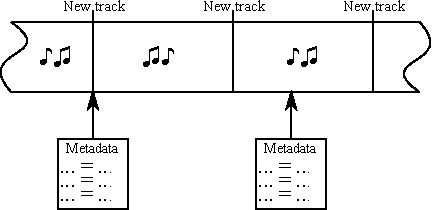
\includegraphics{stream}
\end{center}
 \caption{A \liquidsoap{} stream}
 % Stream.png: 500x132 pixel, 91dpi, 14.03x3.70 cm, bb=0 0 398 105
\end{figure}

The timing, or clock, associated to a multimedia stream can be real-time, if the stream is created 
% DB scaled?
or broadcasted live, or any scaled timing, for instance if the stream consists of files. \textit{A priori},
describing and broadcasting a stream implies real-time output. As we see later, this is unfortunately 
not sufficient for complex settings.
Also, a stream can be finite or infinite. Infinite streams are particularly interesting for broadcasting
because most of the time, we expect a radio, for instance, to be always online. However, this needs 
a special care since it implies some assumption about the validity of the elements that build the stream.

Because streams are infinite objects, they cannot be fully instantiated in memory. Hence, it is 
more appropriate to think of a \textit{stream generator} than of a stream itself which is how
a stream is created in \liquidsoap{}. A stream generator, in \liquidsoap{}, is described as 
an acyclic oriented graph. The edge of the graphs represent the operators, used to create and modify
a stream, while the vertices represent the connections between them.

\subsection*{Stream generation}

Given an acyclic graph describing a stream generator, the roots of the graph are the operator that create 
the initial streams, called \textit{sources}. Those sources can be created from a single file, a playlist, an HTTP input,
the sound card, etc. The sources are then modified and composed with each other using 
\textit{operators} that, for instance, play a source if it is available or a second one otherwise, or modify
the metadata, mix the audio data of two sources, etc.
Finally, the leaves of the graph describe the \textit{outputs} of the stream. Those outputs consist, for instance,
% DB first occurrence of icecast, never introduced
of playing the stream on the local sound card, saving it to a file or sending it to and Icecast server. 
For this initial description, we suppose that the graph has only one output.

As explained, the graph is a \textit{stream generator}. Hence, once the graph has been instantiated,
it is used to generate the stream in the following way: a elementary chunk of data, called a frame, is given to be filled to the 
output operator, the leave of the graph, assumed to be unique for now. 
The output passes the frame to the underlying operators to fill it. Those operators, in turns, pass the frame to their 
underlying operators, until the frame reaches a root node, \ie\ a source. 
Then, the source fills the frame and sends it back to the operator above, which in turn performs
the modifications it has to do, until a filled frame is returned to the output.

\begin{figure}[htn]
 \begin{center}
\[
\xymatrix{
  *+[F]{\mathtt{input.http}}\ar[r]&*+[F]{\mathtt{fallback}}\ar[r]&
  *+[F]{\mathtt{normalize}}\ar[r]&
  *+[F]{\mathtt{output.icecast}}\\
  *+[F]{\mathtt{playlist}}\ar[ur]&\\
}
\]
\end{center}
 \caption{A stream generator}
 % Stream.png: 500x132 pixel, 91dpi, 14.03x3.70 cm, bb=0 0 398 105
\end{figure}

Using this method, the stream can be described using a finite amount of memory. In fact, the frames used
to generate the stream can be statically allocated and passed as memory pointers during the generation, which 
avoids copying data in memory. Also, the stream generator can be used at any rate. For instance,
for a live broadcast, the generator will be asked to fill frames at real rate, while 
for a stream saved to a file, the generator will be asked to fill frames at the maximal possible rate.

Finally, the information of whether or not a stream can be assumed to be infinite is also carried by the 
graph. For instance, if a source is created from a single file, one can try to decode it before starting 
streaming. If the file can be decoded, and one can assume that the file will not be deleted later, and then 
the source can be considered infallible. Later on, if this source is used, for instance in an operator that plays 
the first available source, then the source resulting of this operator is also infallible.
By induction over the vertices of the graph, each node can be considered fallible or not. Eventually,
an infallible output can be considered as describing an infinite stream, while a fallible
output describes a stream that may not be infinite.

\subsection*{Stream sharing}

The description of a stream generator in the previous section is simple and 
natural. Unfortunately, most of the time it is too limited. For instance, one 
may want to have several outputs of the same 
stream, \eg\ one to a local file for archiving purposes and another one to an Icecast server to be
broadcasted.
In this case, the two outputs in the graph are connected to the same operator. Hence, when those output
transmit their frame to this operator to be filled, the operator should fill them with the same data.

\begin{figure}[htn]
 \begin{center}
\[
\xymatrix{
  *+[F]{\mathtt{input.http}}\ar[r]&*+[F]{\mathtt{fallback}}\ar[r]&
  *+[F]{\mathtt{normalize}}\ar[r]\ar[dr]&
  *+[F]{\mathtt{output.icecast}}\\
  *+[F]{\mathtt{playlist}}\ar[ur]& & & *+[F]{\mathtt{output.file}}\\
}
\]
\end{center}
 \caption{A stream generator with caching}
 % Stream.png: 500x132 pixel, 91dpi, 14.03x3.70 cm, bb=0 0 398 105
\end{figure}


For this reason, the first time that the operator is asked to fill the frame, it should pass it to its 
underlying operators, as described before. However, the second time, it should just fill the frame 
with the data gathered during the first call, which implies \textit{caching} the data obtained during the first call.

Therefore, even though the initial stream generator model could avoid copying data in memory, there 
are situations where it is not possible. In order to deal with these situations, the 
model carries a notion of \textit{ticks}. Ticks represent an elementary unit of time
for stream generation. Each frame contains a fixed number of ticks and the stream is split
in bunches of ticks representing each frame. During the same bunch of ticks, when filling a frame, the nodes only 
transmit their frame to their underlying nodes once and, for the successive calls, use a cache of this data. 
Once all the filling operations have been done for a bunch of ticks, the nodes are informed that the 
stream has moved to the next bunch and reset their cached values. 

Finally, the necessity for a node to cache its current frame is detected when instantiating the graph, thus
copying data in memory only when it is necessary.

\subsection*{Stream clocks}

% DB in the following, confusion between transition and crossing

Another limitation of the current model is the possibility to describe advanced transitions in 
the stream. For instance, one may want to use a crossfade between two tracks 
of the stream, \ie{}
fade out the volume of an ending track, fade in the volume of a starting track and merge this together.

\begin{figure}[htn]
 \begin{center}
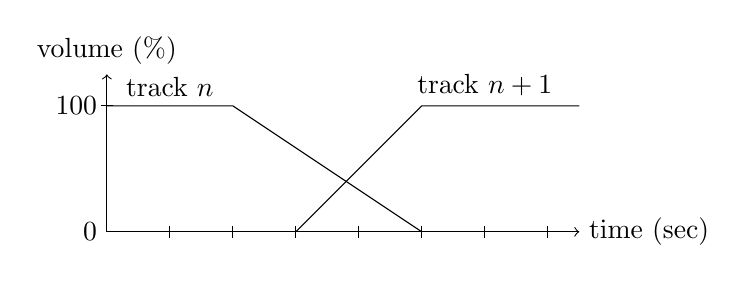
\begin{tikzpicture}[xscale=0.8,yscale=0.8]
\draw[->] (0,0) -- (0,2.5);
\draw (-0.1,2) -- (0.1,2);
\draw (0,2) node[anchor=east]{100};
\draw (0,0) node[anchor=east]{0};
\draw[->] (0,0) -- (7.5,0);
\foreach \x in {1,2,3,4,5,6,7} \draw (\x,-0.1) -- (\x,0.1);
\draw (0,2.5) node[anchor=south]{volume (\%)};
\draw (7.5,0) node[anchor=west]{time (sec)};
\draw (0,2) -- (2,2) -- (5,0);
\draw (3,0) -- (5,2) -- (7.5,2);
\draw (1,2) node[anchor=south]{track $n$};
\draw (6,2) node[anchor=south]{track $n+1$};
\end{tikzpicture}
\end{center}
 \caption{A crossfade transition between two tracks}
 \label{cross-fig}
 % Stream.png: 500x132 pixel, 91dpi, 14.03x3.70 cm, bb=0 0 398 105
\end{figure}

The initial source can be created, for instance, with a playlist of files. Then,
a \texttt{crossfade} operator would take this source and return a source whose tracks are 
crossfaded as shown in Figure \ref{cross-fig}. In order to do this, the operators has to 
detect sufficiently in advance the end of the current track, collect the data of the
end of the track, collect the data of the beginning of the next track, apply the respective
fade out and fade in and add the two streams to create the transition.

However, in this case we need to introduce a new notion in the model. Without transitions, the 
source generator can be used with a uniform rate on all nodes: frames are filled
at the same rate on every node. Unfortunately, the \texttt{crossfade} operator
does not have this property: when it detects the end of a track, it will query many frames in advance 
to the underlying source in order to compute the crossfade. This behaviour breaks the uniformity of 
timing in the graph and requires to introduce \textit{multiple clocks}.


\begin{figure}[htn]
 \begin{center}
\[
\def\f{\save
*+<15pt>[F--]\frm{}\ar @{--} "2,2"\restore}%
\def\g{\save
"2,4"."1,2"."1,5"!C*+<27pt>[F--]\frm{}\ar @{--} "1,1"\restore}%
\xymatrix{
   \mathtt{clock_1} & *+[F]{\mathtt{playlist}}\ar[r]\f&*+[F]{\mathtt{crossfade}}\ar[r]&  *+[F]{\mathtt{fallback}}\ar[r]&
  *+[F]{\mathtt{output.icecast}}\\
   &\mathtt{clock_2} &  & *+[F]{\mathtt{jingles}}\ar[u]\g& 
}
\]
\end{center}
 \caption{A stream generator with different clocks}
 % Stream.png: 500x132 pixel, 91dpi, 14.03x3.70 cm, bb=0 0 398 105
\end{figure}

Clocks are represented in the model by a notion of locality in the graph. The graph is then partitioned into 
different sets, where each set shares the same clock.
When instantiating the graph, each operator declares if it needs a custom clock for him or its sources. 
Then, when initializing the graph of the stream generator, the clocks are attributed by a constraint 
satisfaction algorithm. Because of caching, we do not want a source to be connected to two different operators with 
two different clocks. In this case, this is detected when instantiating the graph and an error is raised.
Similarly, some sources do not support clocks whose rate is different than real time, for instance input 
from the local sound card. In this case too, if the clock attached to the source is not real time, an error
is raised.



\section{The \liquidsoap{} language}
\label{sec:lang}

The \liquidsoap{} language is the formal tool developed to describe the graph of the
stream generator of our model.

\subsection{Syntax}

This part is independent of the target application, \ie\ streaming.
We could use an extension of $\lambda$-calculus instead of our calculus with
multi-application. This would save some space, simplify the operational 
semantics and types.

\subsection{Types}

Types are specific to liquidsoap, starting with content kinds and types.

Type inference, stream kinds and encoding formats.

Theorems: easy if we stick to unary abstractions,
transitivity and reflexivity of subtyping, subject reduction,
even normalization\ldots the only trick is constraints.

\subsection{Static analysis}

\subsubsection{Infallibility}
\subsubsection{Clock assignment}

\subsection{Other remarks}

Documentation, errors, user friendliness.

\bibliographystyle{abbrv}
\bibliography{biblio}
\end{document}
